%!TEX root = report.tex
\exercise{Opening by reconstruction}
A connected component of a logical image can be reconstructed by using geodesic dilation.

Geodesic dilation works by starting out with a \emph{marker image} \texttt{f} with some pixels.
These pixels must be inside one of the connected components of the original image; it marks the connected component.

A larger portion of the connected component is retrieved by dilating the marker image.
However, the dilation might cause the pixels outside of the connected component to be filled, so the intersection with the original image (the mask image \texttt{mask}) has to be taken afterwards, to prevent this.

\texttt{f} and \texttt{mask}, along with the structuring element \texttt{se} that should be used for the dilation are the input arguments for the function \texttt{IPrecon\_by\_dilation}:
\matlabexternal{../IPrecon_by_dilation.m}

\subsection*{Standard opening}
Opening is an operation that can be used for filtering noise from an image.
The standard method works by first eroding the image and then dilating the result of that.
The opening operation is implemented in the \texttt{IPopen} function:
\matlabexternal{../IPopen.m}

Figure~\ref{fig:angio_and_noisy} shows the original non-noisy angiogram and the angiogram with simulated noise.

\begin{figure}[htb]
 \centering
 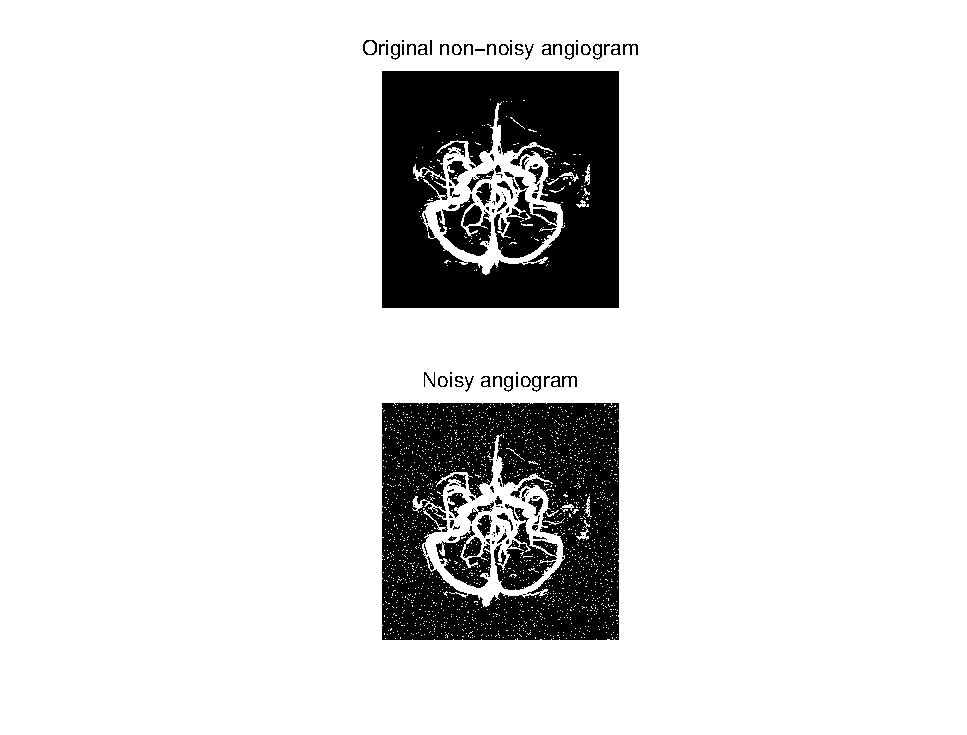
\includegraphics[width=\linewidth]{angio_and_noisy.eps}
 \caption{The original non-noisy angiogram and an angiogram with simulated noise.}
 \label{fig:angio_and_noisy}
\end{figure}

To surpress the noise, the standard opening operation is performed on the noisy-image.
Figure~\ref{fig:angio_open} shows the result, along with the difference with the original non-noisy image.
\(2001\) pixels are still incorrect, when compared with the original non-noisy image.
It can be seen that some parts of the angiogram that are not part of the noise are removed in this process.

\begin{figure}[htb]
 \centering
 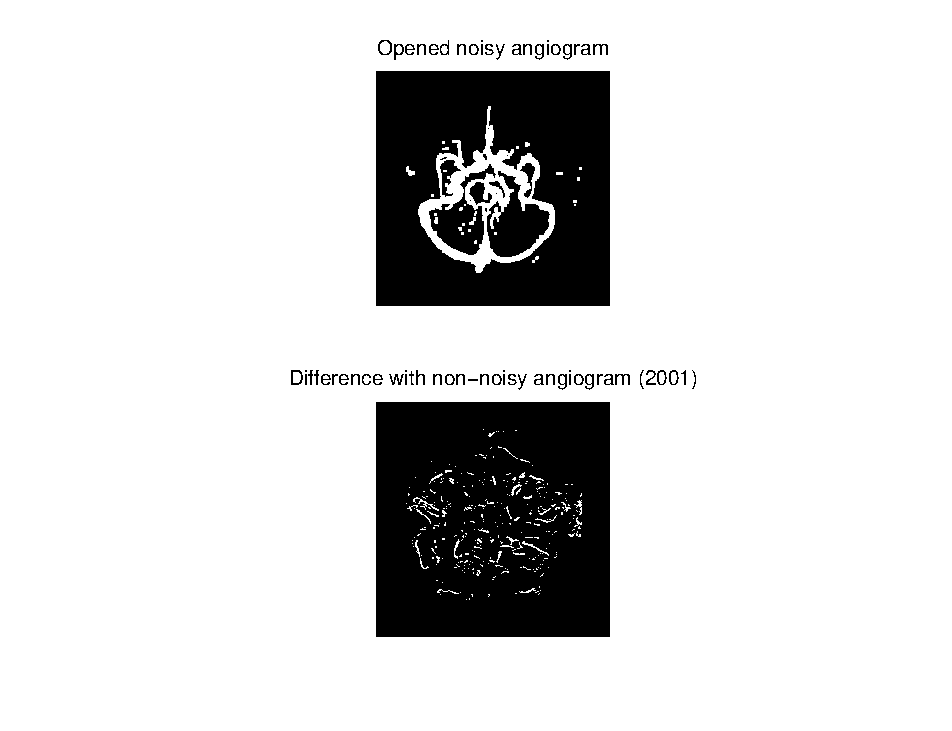
\includegraphics[width=\linewidth]{angio_open.eps}
 \caption{Denoising of an angiogram using normal opening}
 \label{fig:angio_open}
\end{figure}

\clearpage

\subsection*{Alternative opening}
Geodesic dilation can be used for an alternative method of opening.
Just like the standard opening method, the image must first be eroded.
After that, the result is passed as the marker image in the \texttt{IPrecon\_by\_dilation} function.

The original \textbf{noisy} image is passed as the mask.
As a consequence of this, the resulting image can not have any white pixels on places that were not white in the noisy image.\footnote{Note that this fact is the reason that this method only works when there is noise in the \emph{background} of the image and not in the \emph{foreground}. That is, when the ideal non-noisy image is a subset of the noisy image.}

Figure~\ref{fig:angio_open_recon} shows the result of this alternative method, along with the difference with the original non-noisy image.
Only \(665\) pixels are still incorrect, when compared with the original non-noisy image.
This is a major improvement on the standard opening method.
In addition to this, it can be seen that many of the non-noisy parts of the noisy image are retained.

\begin{figure}[htb]
 \centering
 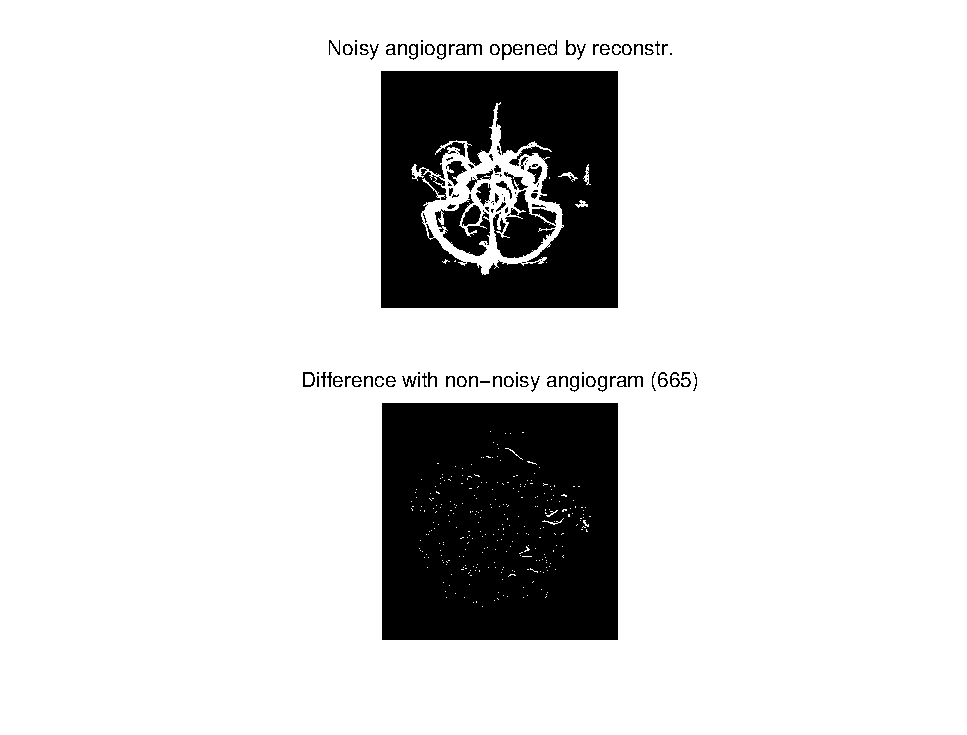
\includegraphics[width=\linewidth]{angio_open_recon.eps}
 \caption{Denoising of an angiogram using opening by reconstruction}
 \label{fig:angio_open_recon}
\end{figure}
\clearpage